\chapter{Working in a simulated environment}

\noindent\begin{wrapfigure}[16]{r}{0.3\textwidth}
    % \captionsetup{singlelinecheck = false, format= hang, justification=raggedright, labelsep=space}
    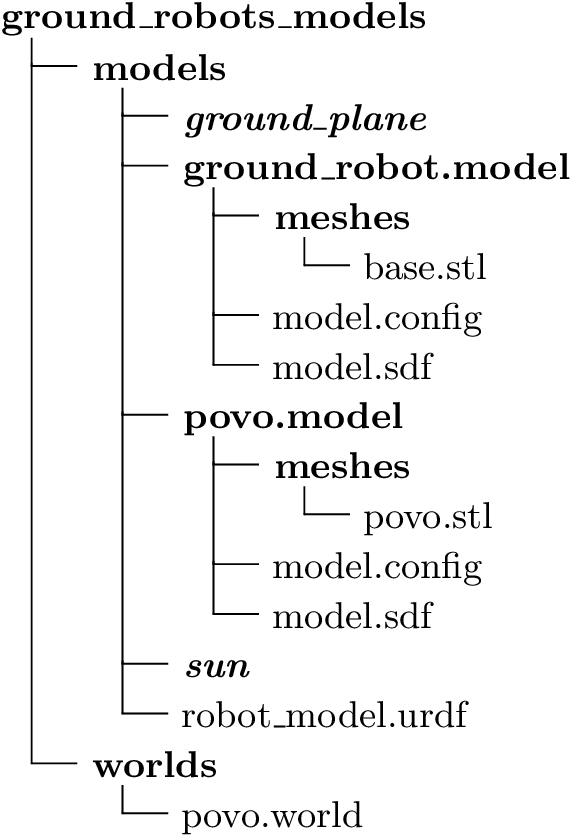
\includegraphics[width=0.3\textwidth]{images/models_folder}
    \caption{Models folder}
\end{wrapfigure}
The choice to develop a \textbf{simulation} is due to the fact that sometimes you may not physically be in the university to use the real robot. The challenge here is doing a good job with the \textbf{abstraction}, which means that the simulated environment and the simulated robot should be \textbf{as close as possible} to real ones. In other words, everything that was working before (i.e. navigation and planning) should now continue to work even if you are no longer in the real world; in theory you should not notice if you are in the real world or in a simulated one.

\section{Models}

In order to create a complete simulation, we need to create what is missing from the reality, which are the models of the environment and the robot.

\subsection{Environment}
\label{sub:map}

A mesh of the Povo upper floors was provided by professor \textit{Marco Roveri} \cite{roveri}. Unfortunately, when compared to the navigation map generated from real data, it turns out that the mesh is \textbf{not very accurate}. Two workarounds are possible: creating a \textbf{new navigation map} for simulation purposes or \textbf{adapting the mesh} as much as possible (?); it turns out, as described in \autoref{sub:waypoints}, by scaling the mesh \textbf{1.0925 times} in the long direction leads to a better result. % testare slam con mesh e fare nuova mappa
Then a model is creating using \acrfull{sdf}, with the mesh employed in \textbf{visual} and \textbf{collisions} tags (?); this model is then used in \code{world} file\footnote{Always written in \acrshort{sdf}} (alongside with ground plane and sun ones, provided by Gazebo and the robot model, of course).

\begin{figure}[h]
    \centering
    \includegraphics[width=0.8\textwidth]{images/3d\_povo\_model}
    \caption{Povo model for simulation. Colors were used for a better visualization.}
\end{figure}

\subsection{Robot}

Part of the setup is inspired to Automatic Addison tutorials\cite{tutorials}. % forse togliere (?)

The robot mesh was created starting from \textit{shelfino} (see \autoref{fig:shelfino}), trying to keep it \textbf{as similar as possible}, and each piece (robot base, lidar, wheels and caster wheel) was exported singularly. For performance reasons in Gazebo, the only mesh actually used is the robot base, because of its special structure to \textbf{avoid contact} with the spinning wheels \textbf{partially inside}. The other ones are substituted by \acrshort{sdf} or \acrfull{urdf} built-in geometric shapes (i.e. cylinders).
Both \acrshort{sdf} and \acrshort{urdf} were used: the first one is used by Gazebo, the second one by a node called \code{robot\_state\_publisher} that helps visualize the robot in \acrshort{rviz}.

\begin{figure}[h]
    \centering
    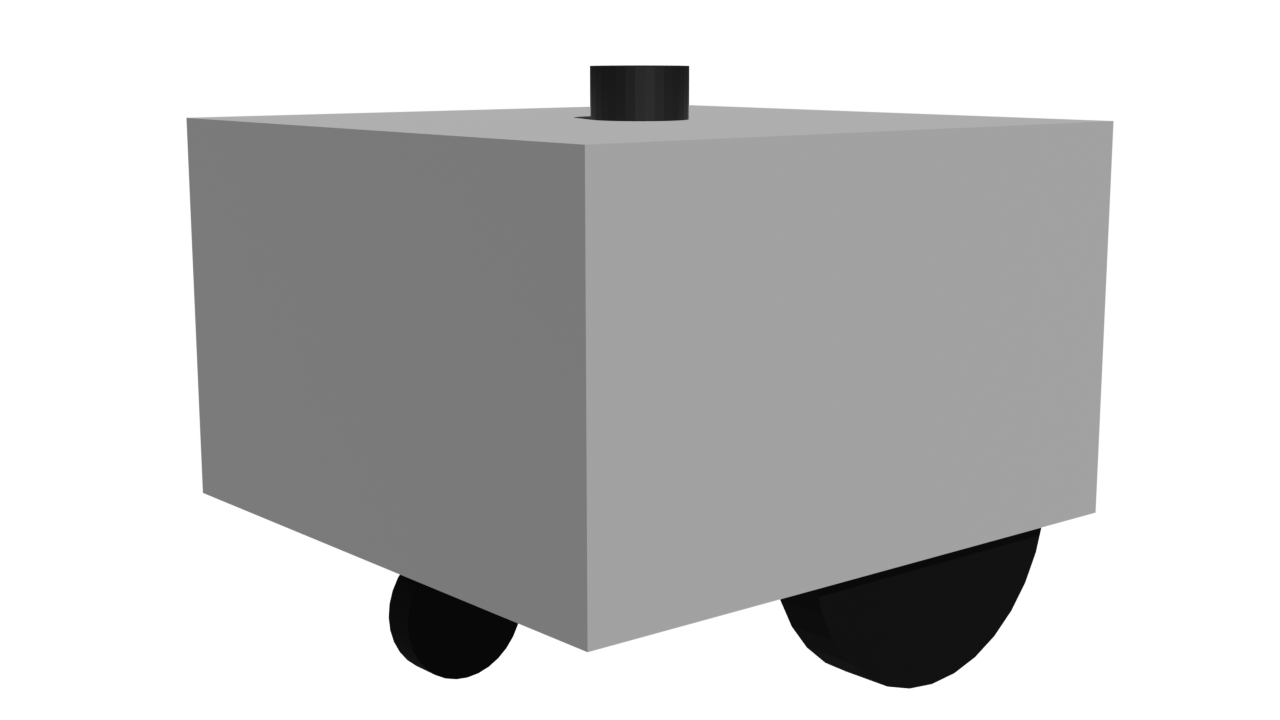
\includegraphics[width=0.7\textwidth]{images/shelfino_3d.png}
    \caption{Shelfino model for simulation.}
\end{figure}

\section{Gazebo plugins}

After placing the models in Gazebo, we need some way to make our robot \textbf{interact} with the environment. It is no longer possible to utilize the nodes in \autoref{subsec:nodes} because they make use of a real hardware, but thankfully Gazebo provides some \textbf{plugins} that can be added to the \acrshort{sdf} model as a normal tag.
We always need a way to set \textbf{linear and angular velocities} to make the robot moves as desired, a way to \textbf{calculate odometry} and a lidar to \textbf{detect obstacles}. Once done, the robot can be used as if it were a real robot.

Sadly, no tracking camera plugins are available, so we content ourselves with only wheel rotation information to calculate odometry. 

\subsection{Differential drive plugin}

Once added, some configurations needs to be made:
\begin{itemize}
    \item set \textbf{update rate} (Hz)
    \item specify \textbf{name} of wheel joints (control)
    \item set wheels \textbf{separation} and \textbf{diameter} (kinematics)
    \item set max \textbf{torque} and \textbf{acceleration} (limits)
    \item specify topic names from where \textbf{receiving desired velocity} and \textbf{publish odometry data}
    \item whether to \textbf{publish frame transformations} and their names (used by \acrshort{rviz})
\end{itemize}
After that, the robot can now move.

\subsection{Joint state publisher plugin} % forse toglierlo (?)

This plugin is used to know how much the wheels are spinning in order to visualize them in \acrshort{rviz}. Only update rate and wheel names are required. (?)

\subsection{Ray sensor plugin}

To be able to detect obstacles, a lidar is needed. To do so, you can just use the \textbf{sensor} tag \code{ray} of Gazebo, setting \textbf{scan}, \textbf{range} and \textbf{noise} information, but also a plugin is required to make it work. Only configurations needed are:
\begin{itemize}
    \item what \acrshort{ros} message type to use as \textbf{output} (\code{sensor\_msgs/LaserScan})
    \item frame name where the lidar is \textbf{attacched} to (described somewhere else in the model)
\end{itemize}

% add robot description of link, joints, ecc...? o qualcos'altro? tipo sdf come allegato? (?)

% aggiungere struttura cartella con models e worlds solo